\documentclass[aspectratio=169]{beamer}
\usepackage[french]{babel}
\uselanguage{French}
\languagepath{French}
\usepackage{hyperref}
\usepackage[T1]{fontenc}

\usepackage{amsmath,amsthm,amssymb,parskip}

\usepackage{multicol}
\usepackage{stmaryrd}
\usepackage{graphicx,float}
\usepackage{hyperref}

% other packages
\usepackage{latexsym,amsmath,xcolor,multicol,booktabs,calligra}
\usepackage{graphicx,pstricks,listings,stackengine}
\usepackage{datetime} 
% dummy text; remove it when working on this template
\usepackage{lipsum}

\usepackage[most]{tcolorbox}

\usepackage{listings}
\usepackage{lstautogobble}
\usepackage{tikz}

\author{Hugo Mouton}
\title{\textit{Generative Art via Grammatical Evolution}}
\subtitle{Présentation d'article}
\institute{
    Polytechnique Montréal
}
\date{\today}
\usepackage{UTU}

% defs
\def\cmd#1{\texttt{\color{red}\footnotesize $\backslash$#1}}
\def\env#1{\texttt{\color{blue}\footnotesize #1}}
\definecolor{utu_green}{RGB}{173,203,0}
\definecolor{ex_green}{RGB}{48,115,34}
\definecolor{utu_blue}{RGB}{93,155,162}
\definecolor{utu_pink}{RGB}{248,72,94}
\definecolor{halfgray}{gray}{0.55}

\newcommand{\Rm}{\mathbb{R}_{\max}}
\newcommand{\R}{\mathbb{R}}

\newtcbtheorem{mytheo}{Theorem}{colback=purple!5,colframe=blue!100!,fonttitle=\bfseries}{th}
\newtcbtheorem{mydef}{Definition}{colback=purple!5,colframe=orange!100!,fonttitle=\bfseries}{def}
\newtcbtheorem{myprop}{Property}{colback=purple!5,colframe=red!100!,fonttitle=\bfseries}{prop}
\newtcbtheorem{myexample}{Exemple}{colback=purple!5,colframe=ex_green!100!,fonttitle=\bfseries}{example}

\lstset{ %
  language=C,
  numbers=left,
  numberstyle=\tiny,
  stepnumber=1,
  numbersep=5pt,
  breaklines=true,
  autogobble=true, % Removes indentation based on first line
}

%%
%% Julia definition (c) 2014 Jubobs
%%
\lstdefinelanguage{Julia}%
  {morekeywords={abstract,break,case,catch,const,continue,do,else,elseif,%
      end,export,false,for,function,immutable,import,importall,if,in,%
      macro,module,otherwise,quote,return,switch,true,try,type,typealias,%
      using,while,struct},%
   sensitive=true,%
   alsoother={\$},%
   morecomment=[l]\#,%
   morecomment=[n]{\#=}{=\#},%
   morestring=[s]{"}{"},%
   morestring=[m]{'}{'},%
}[keywords,comments,strings]%

\lstset{%
    language         = Julia,
    basicstyle       = \ttfamily,
    keywordstyle     = \bfseries\color{blue},
    stringstyle      = \color{magenta},
    commentstyle     = \color{ForestGreen},
    showstringspaces = false,
}

\begin{document}

\begin{frame}
    \titlepage
    \begin{figure}[htpb]
        \begin{center}
            \vspace{-0.5cm}\includegraphics[keepaspectratio, scale=0.5]{fig/Logo_Polytechnique_Montréal.png}
        \end{center}
    \end{figure}
\end{frame}

\begin{frame}{Table of contents}
    \tableofcontents[sectionstyle=show,subsectionstyle=hide]
\end{frame}

\section{Introduction}

\begin{frame}{Contexte}
    \begin{itemize}
        \item \textit{Generative Art via Grammatical Evolution}, 2023 
        \item Présentation de \textit{GenerativeGI}, un framework expérimental de génération d'art
        \item Utilisation de l'Évolution Grammaticale (GE), technique issue des algorithmes génétiques
        \item Pas vraiment d'algorithme mais plutôt une combinaison de techniques artistiques et une optimisation des paramètres
    \end{itemize}
\end{frame}

\section{Concepts clés}

\subsection{Art Génératif}

\begin{frame}{Techniques d'art génératif utilisées}
    Restriction à 7 techniques génératives: 
    \begin{multicols}{2}
        \begin{itemize}
            \item Stipple
            \item Cellular Automata
            \item Pixel Sorting 
            \item Circle Packing 
            \item Flow Field 
            \item Drunkard's Walk 
            \item Dithering 
        \end{itemize}
    \end{multicols}
\end{frame}

\begin{frame}{Techniques d'art génératif utilisées}
    \begin{figure}
        \centering
        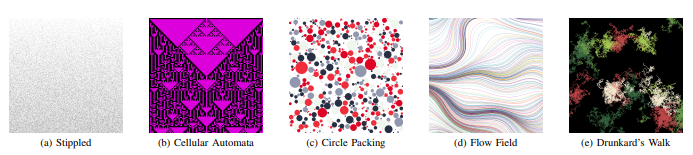
\includegraphics[scale=0.7]{fig/techniques.png}
        \caption{5 des techniques utilisées}
    \end{figure}
\end{frame}

\subsection{Évolution Grammaticale}

\begin{frame}{Qu'est ce que l'Évolution Grammaticale ?}
    \begin{itemize}
        \item Issue des concepts de la programmation évolutive et des algorithmes génétiques
        \item Recherche d'une solution dans un espace contraint par des règles grammaticales établies 
        \item Notion de \textit{génome} = mot de la grammaire choisie 
    \end{itemize}
\end{frame}

\begin{frame}{\textit{Tracery}}
    \begin{itemize}
        \item Framework de génération de texte par application de règles grammaticales
        \item Symboles: les différentes techniques et leurs paramètres
        \item Mots/Génomes: suites de techniques ainsi que leurs paramètres
        \item Nombre limite de transformations dans le cas où il y a peu de symboles terminaux
    \end{itemize}
    \begin{figure}
        \centering
        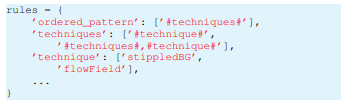
\includegraphics[scale=0.8]{fig/pythonGrammar.png}
        \caption{Représentation Python de la structure de \textit{Tracery}}
    \end{figure}
\end{frame}

\begin{frame}{Mutations de génomes}
    Dans \textit{GenerativeGI}, 2 types de mutations sont autorisées:
    \begin{enumerate}
        \item Sélection d'une technique à un indice aléatoire du génome et remplacement par une autre technique (ou une suite récursive de techniques) \\
        \texttt{flowField('edgy', 0.1)} $\rightarrow$ \texttt{dither('halftone')},\texttt{flowField('edgy', 0.1)}
        \item Modification des paramètres associés à la technique \\
        \texttt{flowField('edgy', 0.1)} $\rightarrow$ \texttt{flowField('edgy', 0.025)}
    \end{enumerate}    
\end{frame}

\begin{frame}{Croisement de génomes}
    Une autre façon de créer de nouveaux individus est le croisement de génomes. \\
    On choisit un symbole aléatoire dans chaque génome et on échange les 2 symboles.\\
    \underline{Génome 1:} \texttt{dither('halftone')},\color{red} \texttt{flowField('edgy', 0.1)} \color{black}\\
    \underline{Génome 2:} \texttt{flowField('edgy', 0.025)},\color{red}\texttt{flowField('edgy', 0.025)} \color{black}\\
    On échange les derniers symboles de chaque génome:\\
    \underline{Nouveau génome 1:} \texttt{dither('halftone')},\color{red}\texttt{flowField('edgy', 0.025)} \color{black} \\
    \underline{Nouveau génome 2:} \texttt{flowField('edgy', 0.025)},\color{red}\texttt{flowField('edgy', 0.1)} \color{black} \\
\end{frame}

\subsection{Sélection de génomes}

\begin{frame}{Lexicase Selection}
    \begin{itemize}
        \item Algorithme de sélection de parents dans les algorithmes génétiques
        \item Choix des parents à une certaine génération pour créer les individus enfants de la prochaine génération 
        \item Algorithme de recherche de solutions dans un espace en utilisant un ensemble de fonctions objectif 
        \item Domaines: programmation génétique, robotiques, géosciences, etc... 
    \end{itemize}
\end{frame}

\begin{frame}{Phase de sélection}
    Déroulement d'une phase de sélection:
    \begin{enumerate}
        \item On récupère un échantillon de la population 
        \item On mélange les fonctions objectifs et on évalue les individus avec la première
        \item Si un individu est meilleur que tous les autres, on le conserve, sinon, on évalue les individus égaux avec la seconde fonction objectif
        \item On répète jusqu'à n'avoir qu'un individu ou s'il n'y a plus de fonctions objectif 
        \item Si il reste des individus égaux selon toutes les fonctions objectifs, un individu est choisi aléatoirement
    \end{enumerate}
\end{frame}

\section{Le framework \textit{GenerativeGI}}

\begin{frame}{Le framework \textit{GenerativeGI}}
    \begin{itemize}
        \item Framework de création d'art génératif par évolution grammaticale 
        \item Prend en entrée une suite de techniques paramétrées 
        \item Génération d'images plus satisfaisantes
        \item Contrôle de la génération en fonction des préférences de l'artiste  
    \end{itemize}
\end{frame}

\begin{frame}{Architecture de \textit{GenerativeGI}}
    \begin{figure}
        \centering
        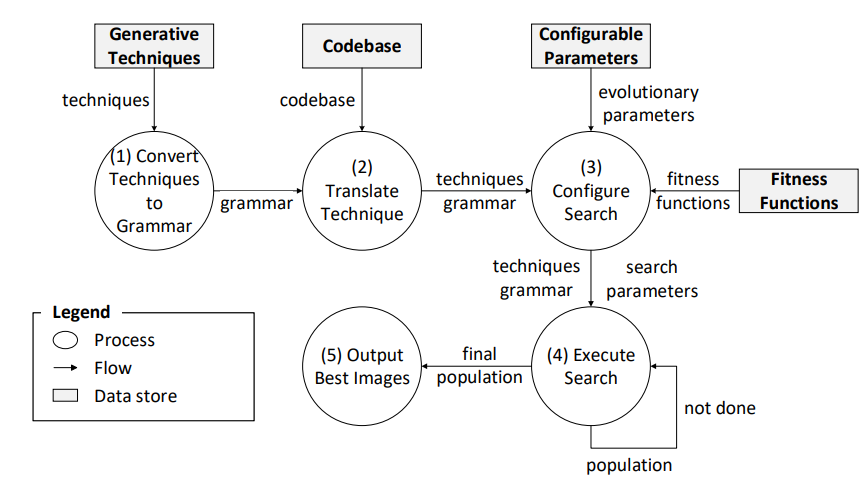
\includegraphics[scale=0.4]{fig/archi.png}
        \caption{Diagramme du fonctionnement de \textit{GenerativeGI}}
    \end{figure}
\end{frame}

\begin{frame}{(1) et (2) Utilisation de Tracery}
    \begin{figure}
        \centering
        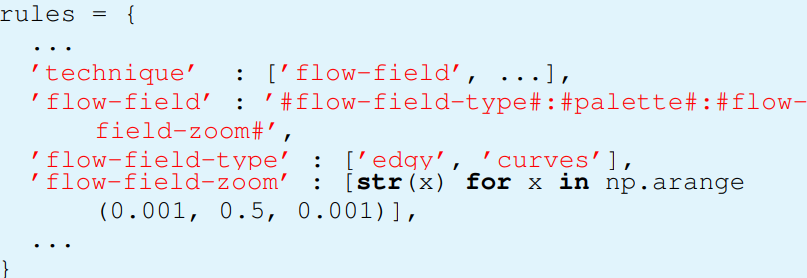
\includegraphics[scale=0.4]{fig/grammar.png}
        \caption{Exemple de conversion grammaticale dans le cas du \texttt{flow-field}}
    \end{figure}
\end{frame}

\begin{frame}{Architecture de \textit{GenerativeGI}}
    \begin{figure}
        \centering
        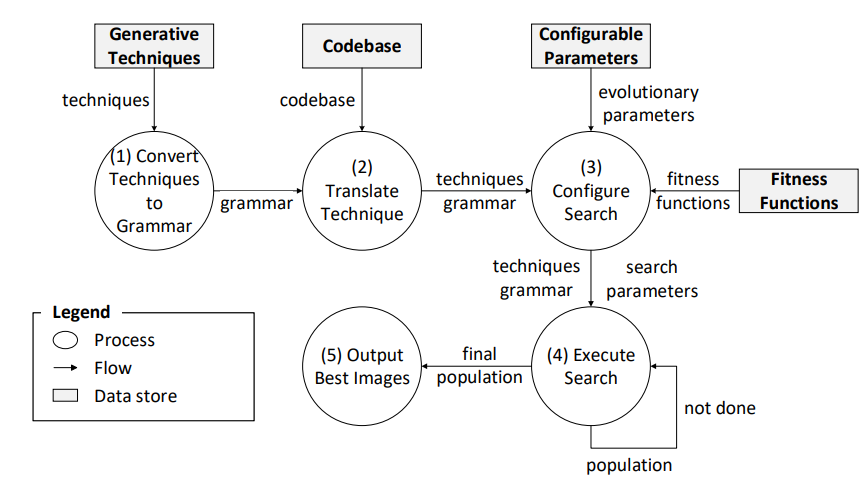
\includegraphics[scale=0.4]{fig/archi.png}
        \caption{Diagramme du fonctionnement de \textit{GenerativeGI}}
    \end{figure}
\end{frame}

\begin{frame}{(3) Configuration de l'espace de recherche}
    
\end{frame}

\section{Résultats}

\begin{frame}{Merci}
    \begin{center}
        Merci de votre attention !
    \end{center}
\end{frame}
    
\end{document}